\subsection{Diccionario de datos}
Descripción de las 25 tablas, nombres de columnas, las ocho variables socioeconómicas y los módulos por examen.

\subsection{Manual técnico}
Manual técnico de despliegue, alineado con las normas ISO aplicables.
	
\subsection{Capturas del tablero interactivo}
\begin{figure}[h]
	\centering
	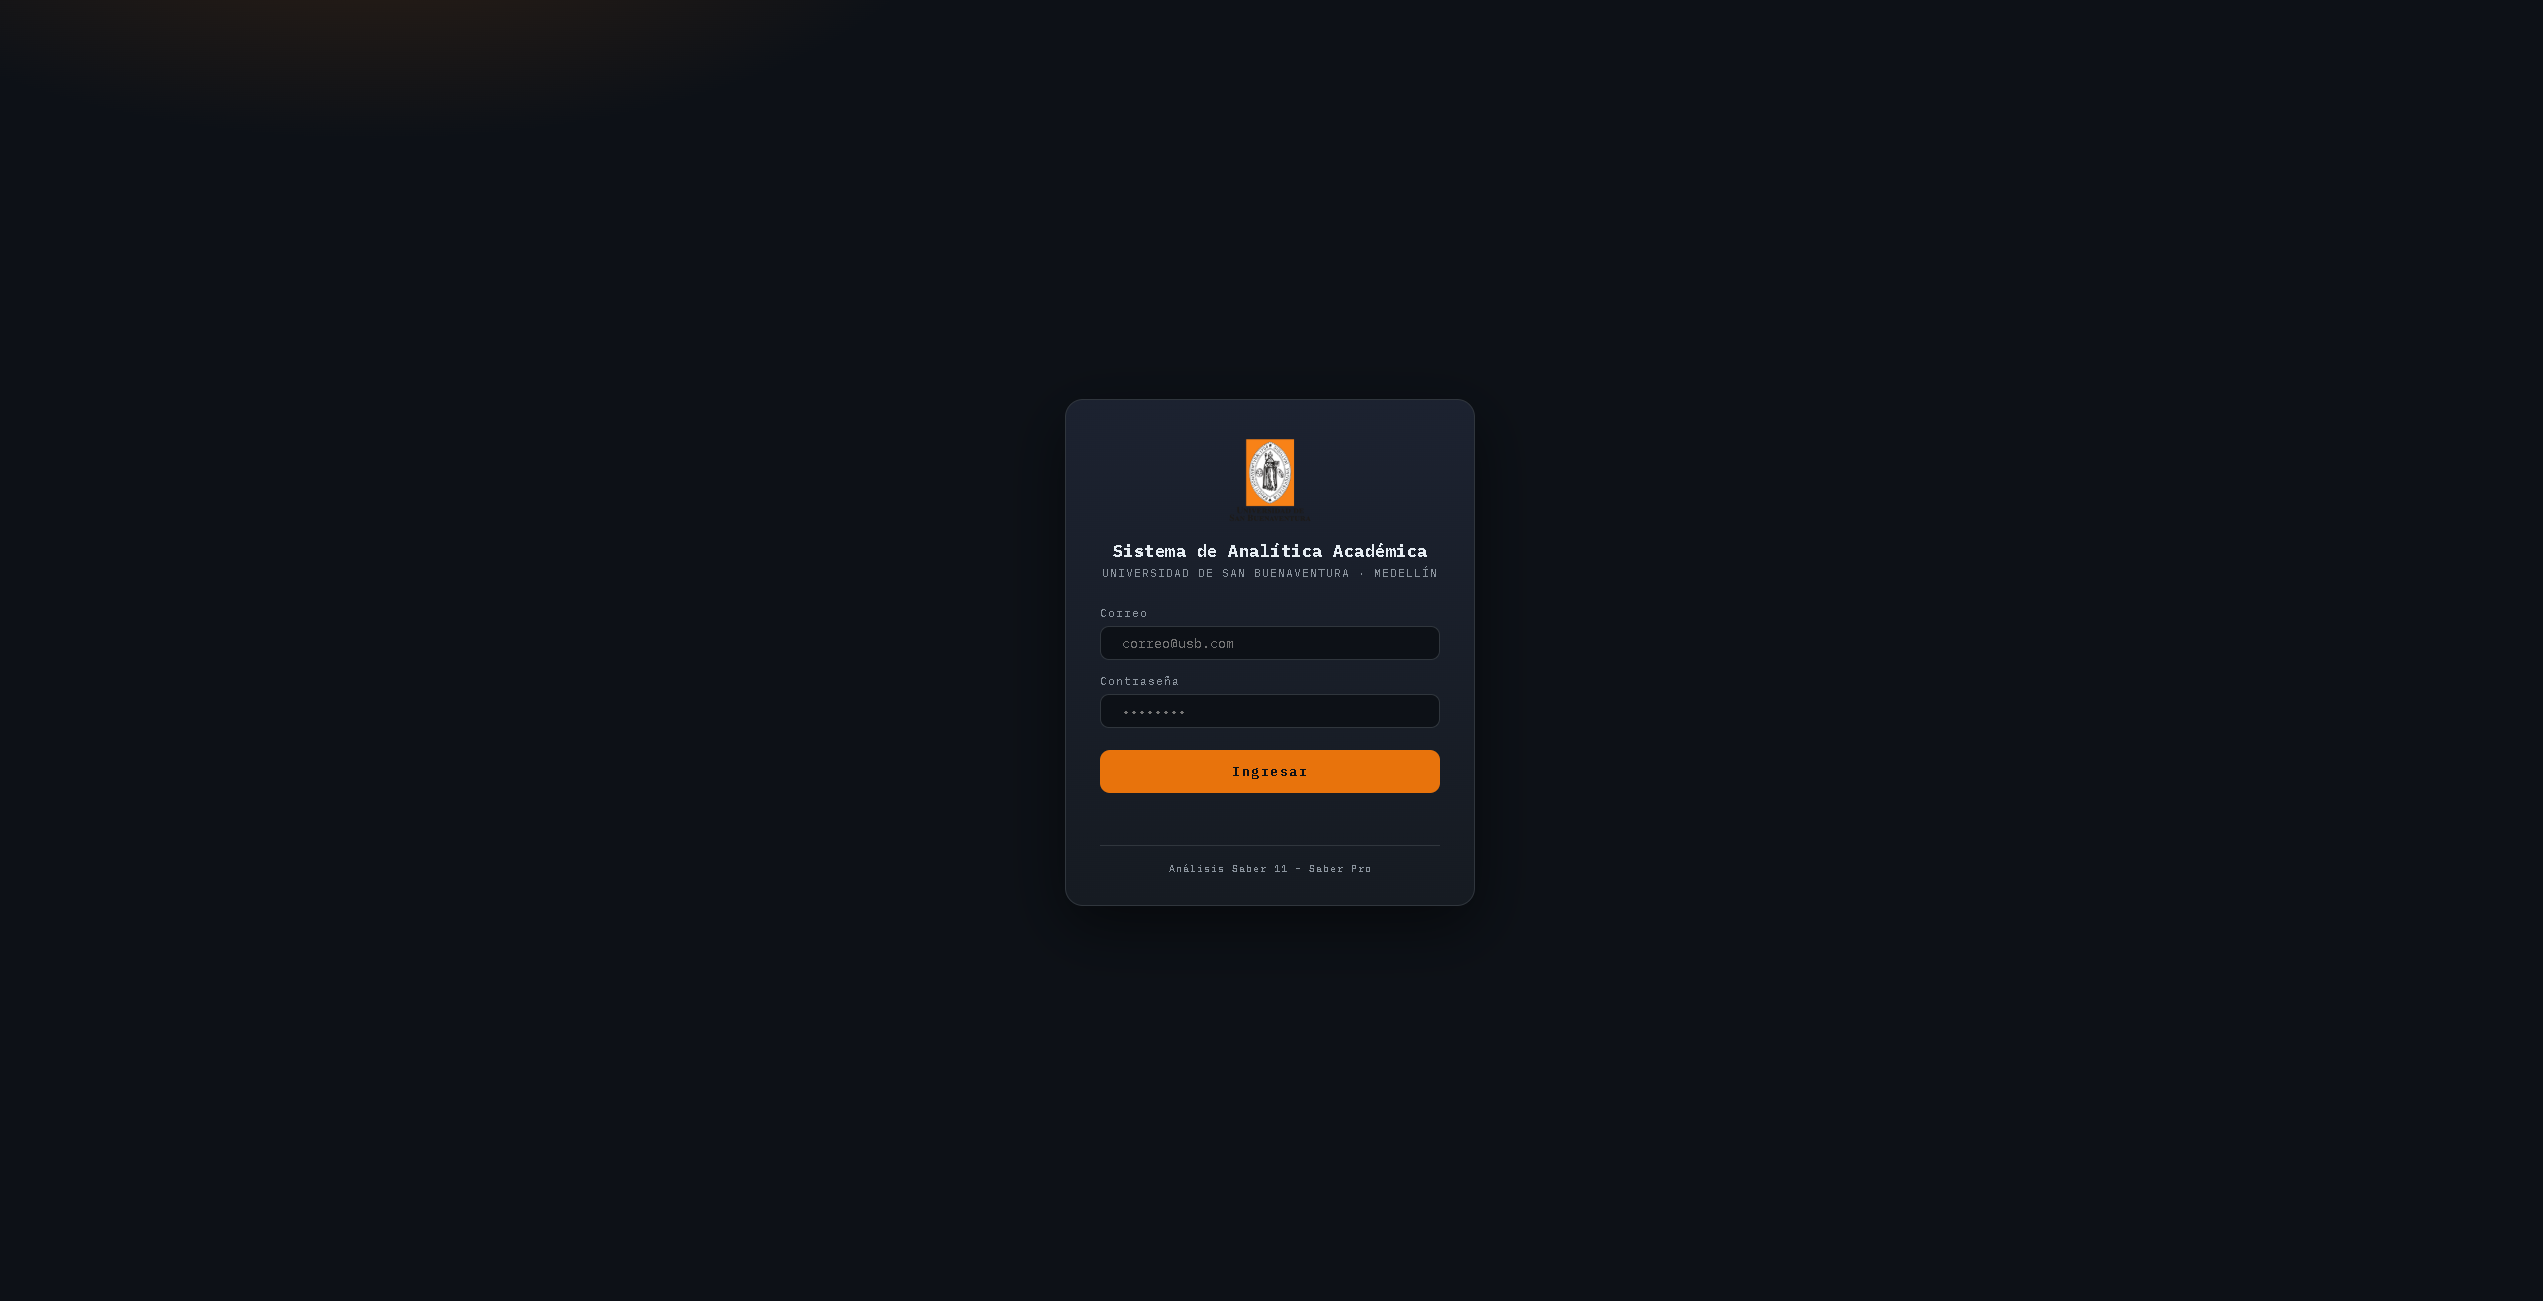
\includegraphics[width=0.7\textwidth]{images/login.png}
	\caption{Menú de login.}
	\label{fig:mi_imagen}
\end{figure}

\begin{figure}[h]
	\centering
	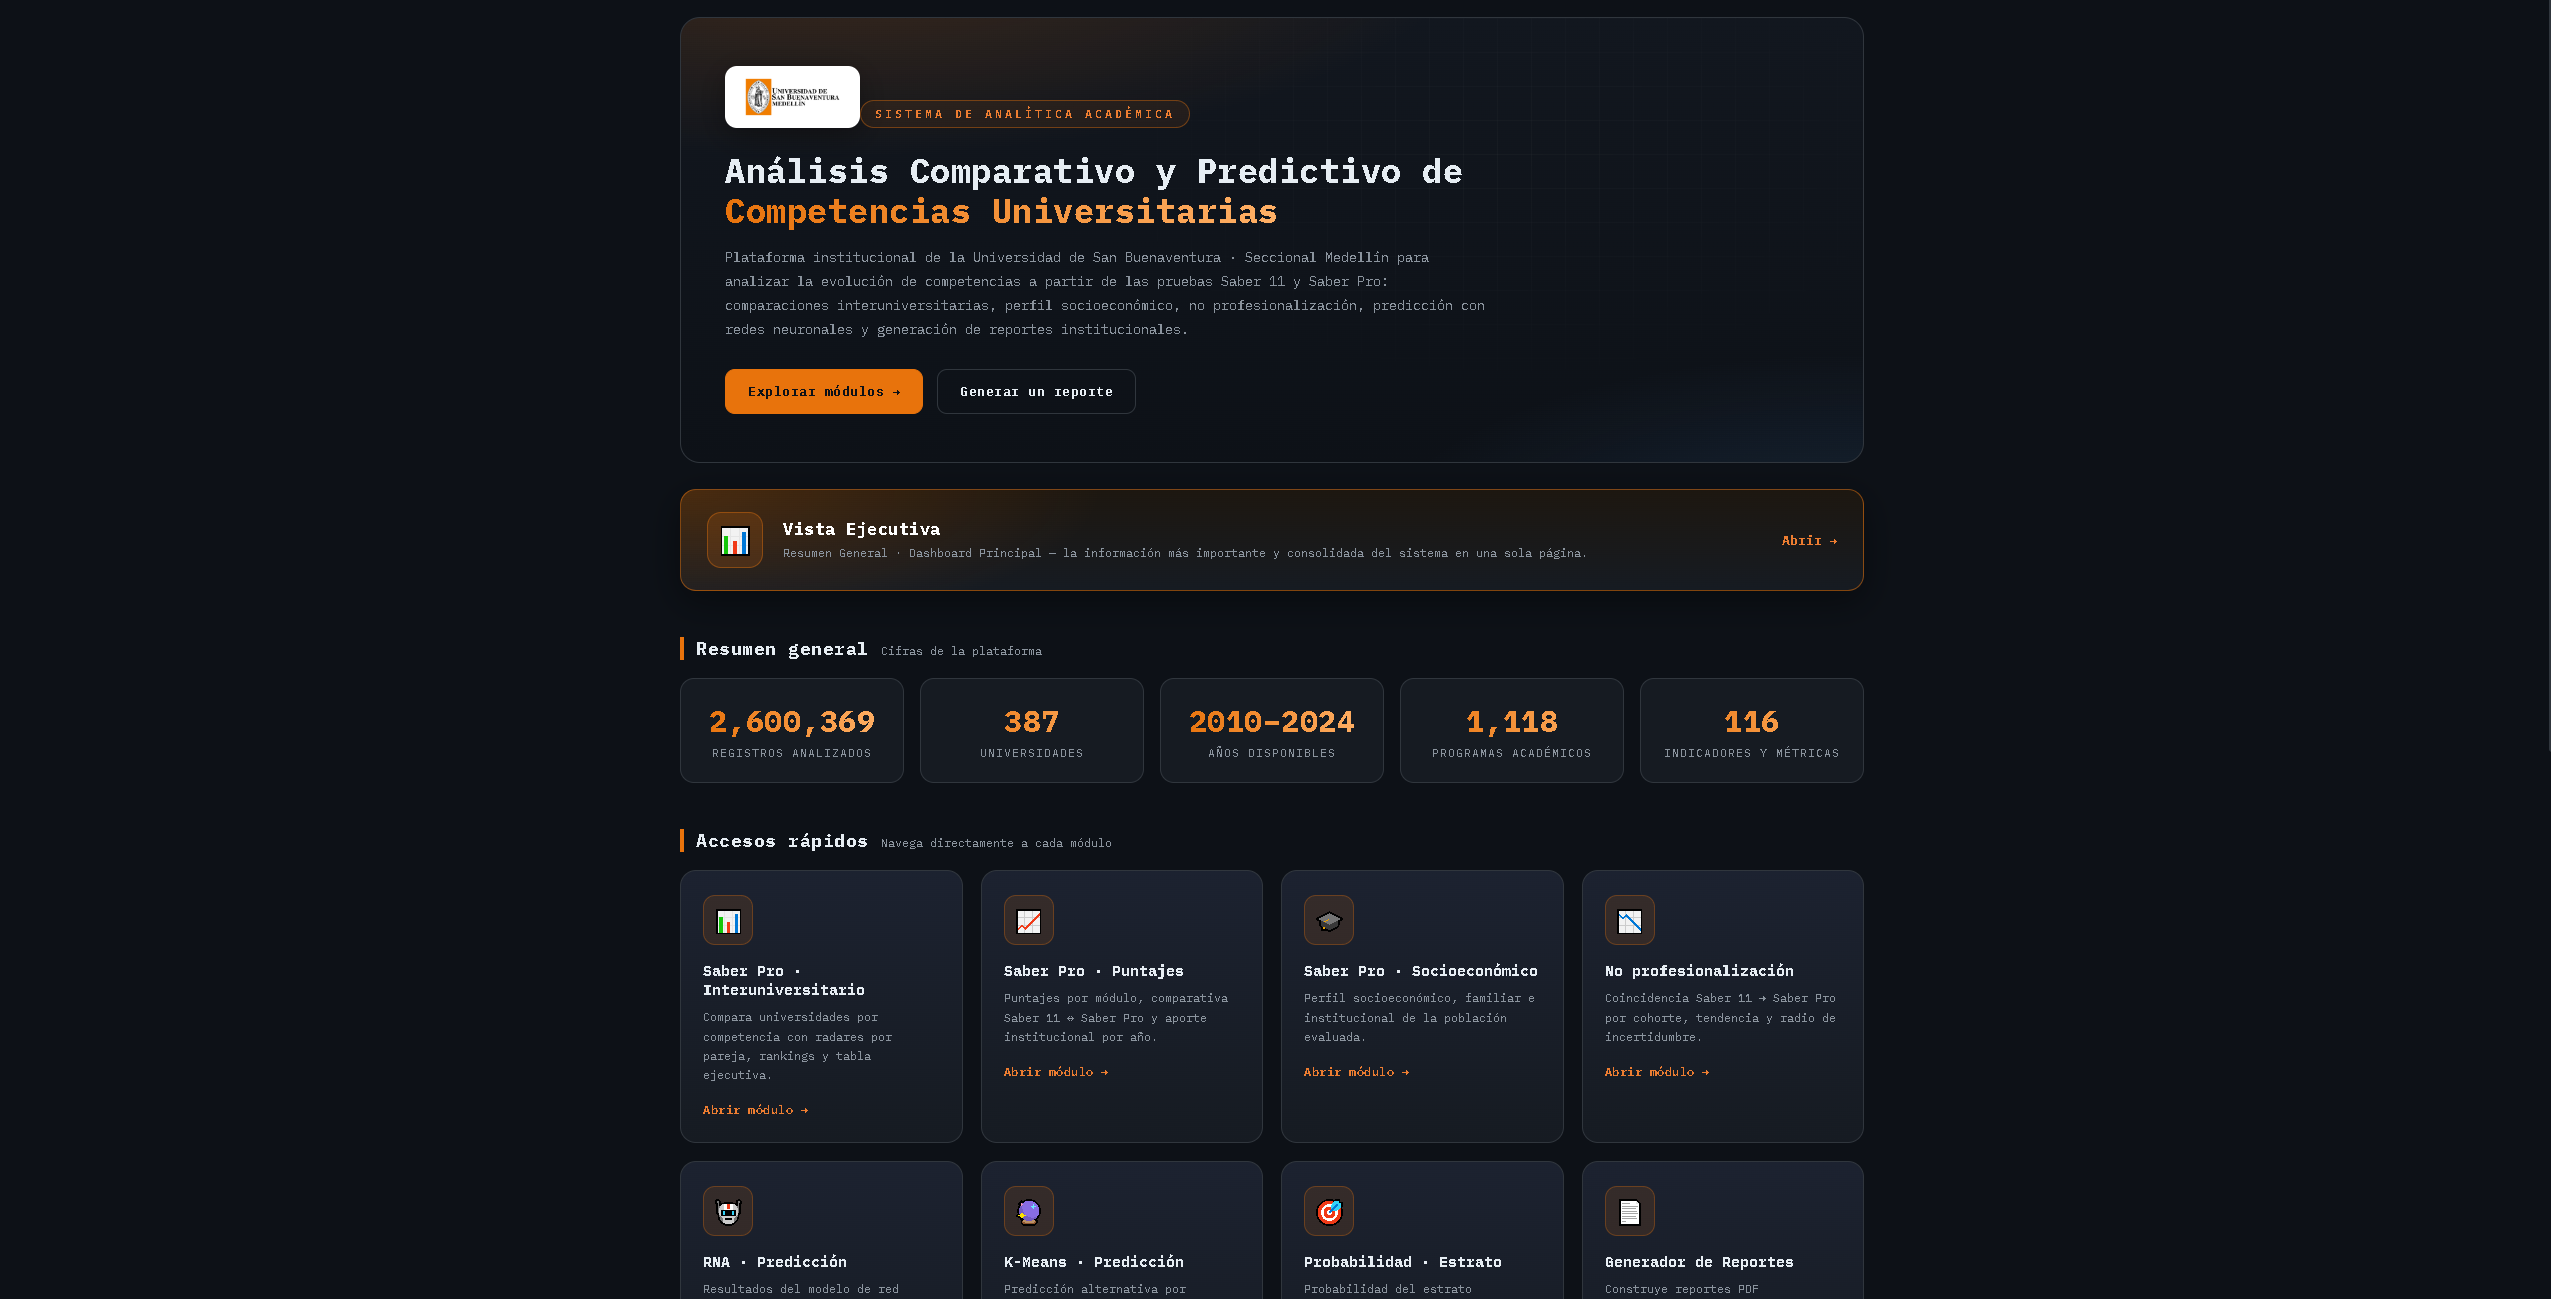
\includegraphics[width=0.7\textwidth]{images/home.png}
	\caption{Página de inicio.}
	\label{fig:mi_imagen}
\end{figure}

\begin{figure}[h]
	\centering
	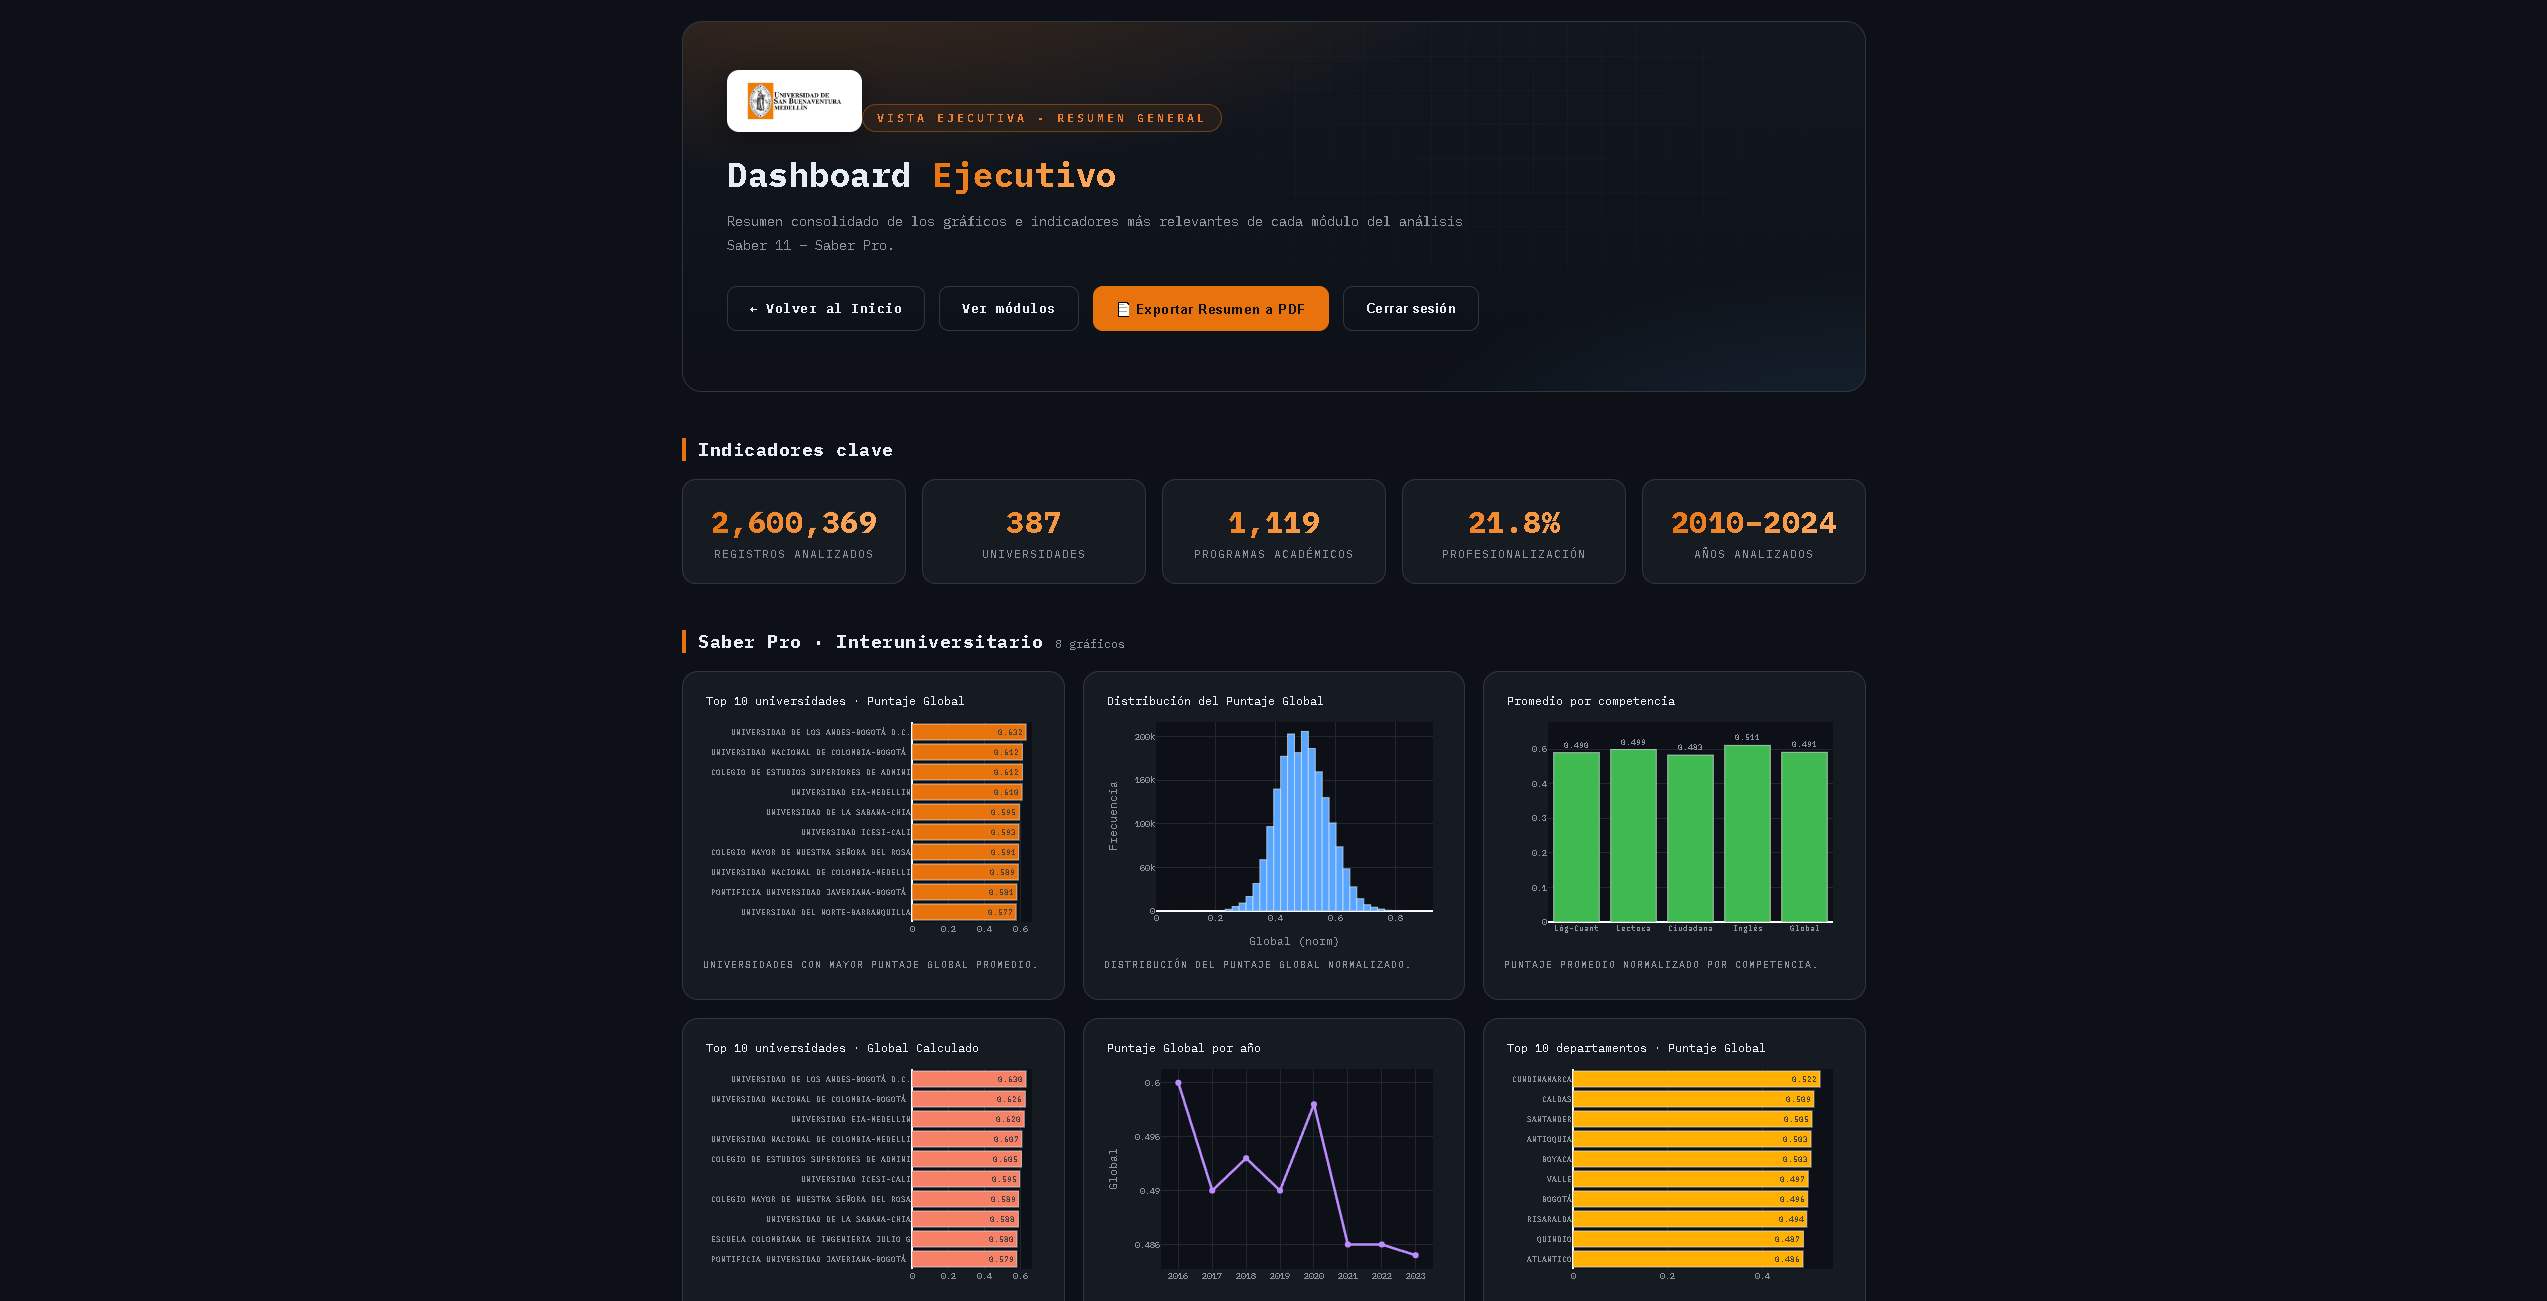
\includegraphics[width=0.7\textwidth]{images/vista_ejecutiva.png}
	\caption{Menú de resumen.}
	\label{fig:mi_imagen}
\end{figure}

\begin{figure}[h]
	\centering
	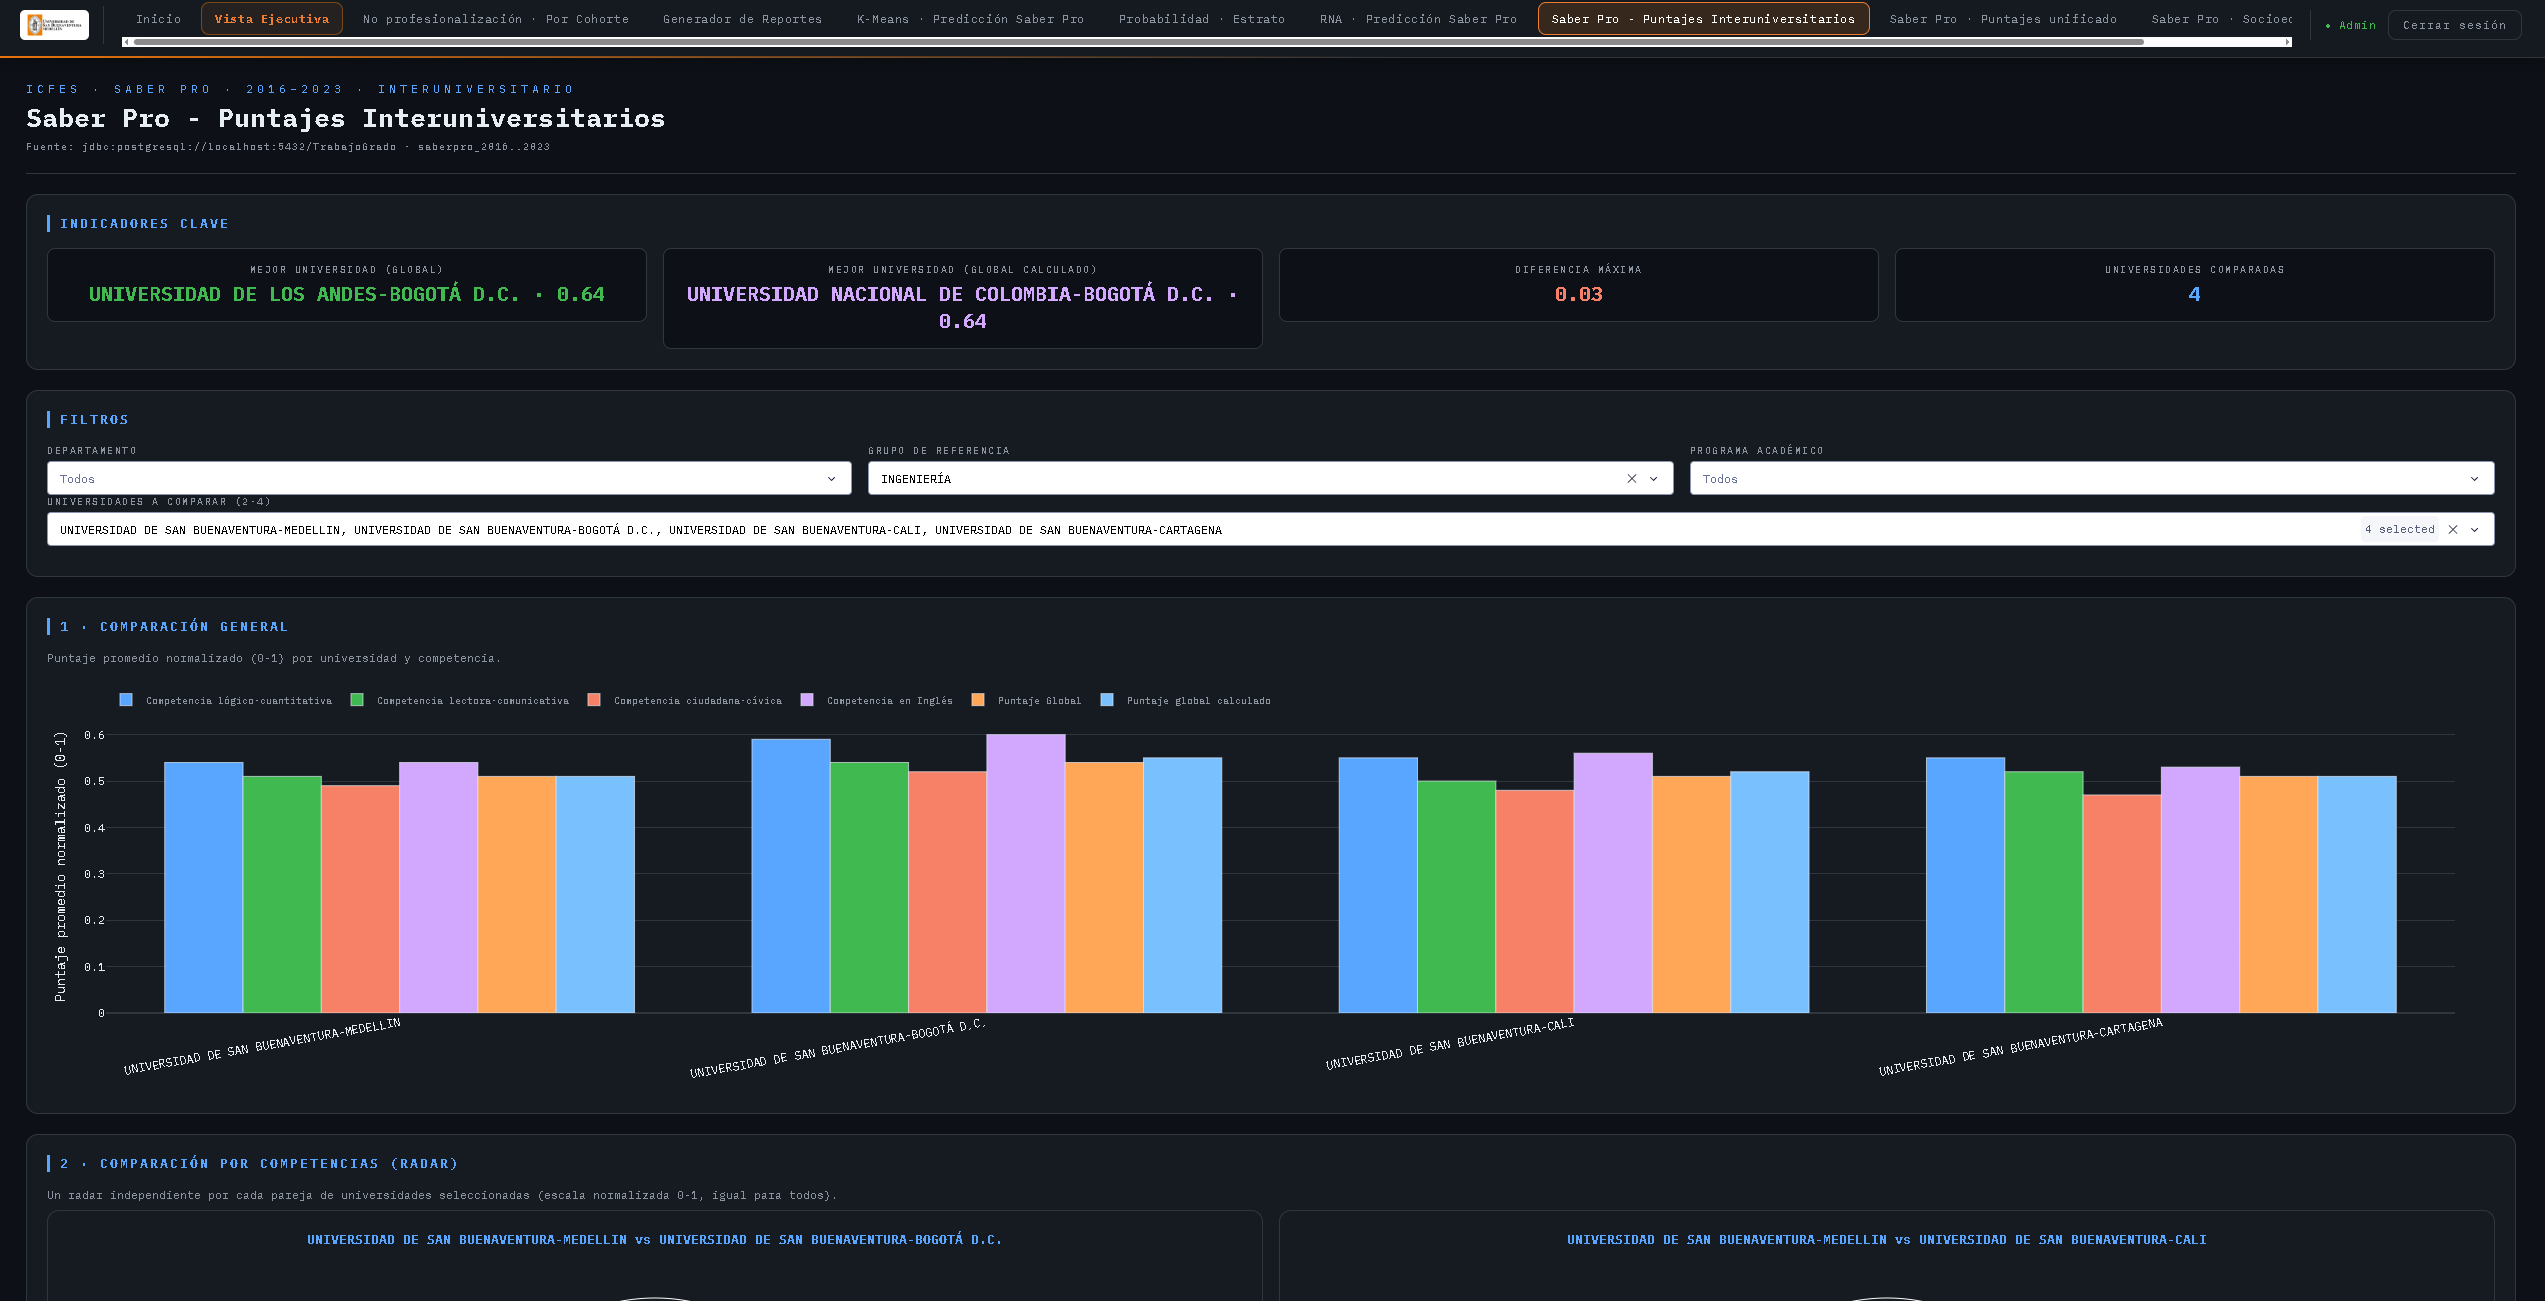
\includegraphics[width=0.7\textwidth]{images/puntajes_interuniv.png}
	\caption{Menú de comparativa para puntajes entre universidades.}
	\label{fig:mi_imagen}
\end{figure}

\begin{figure}[h]
	\centering
	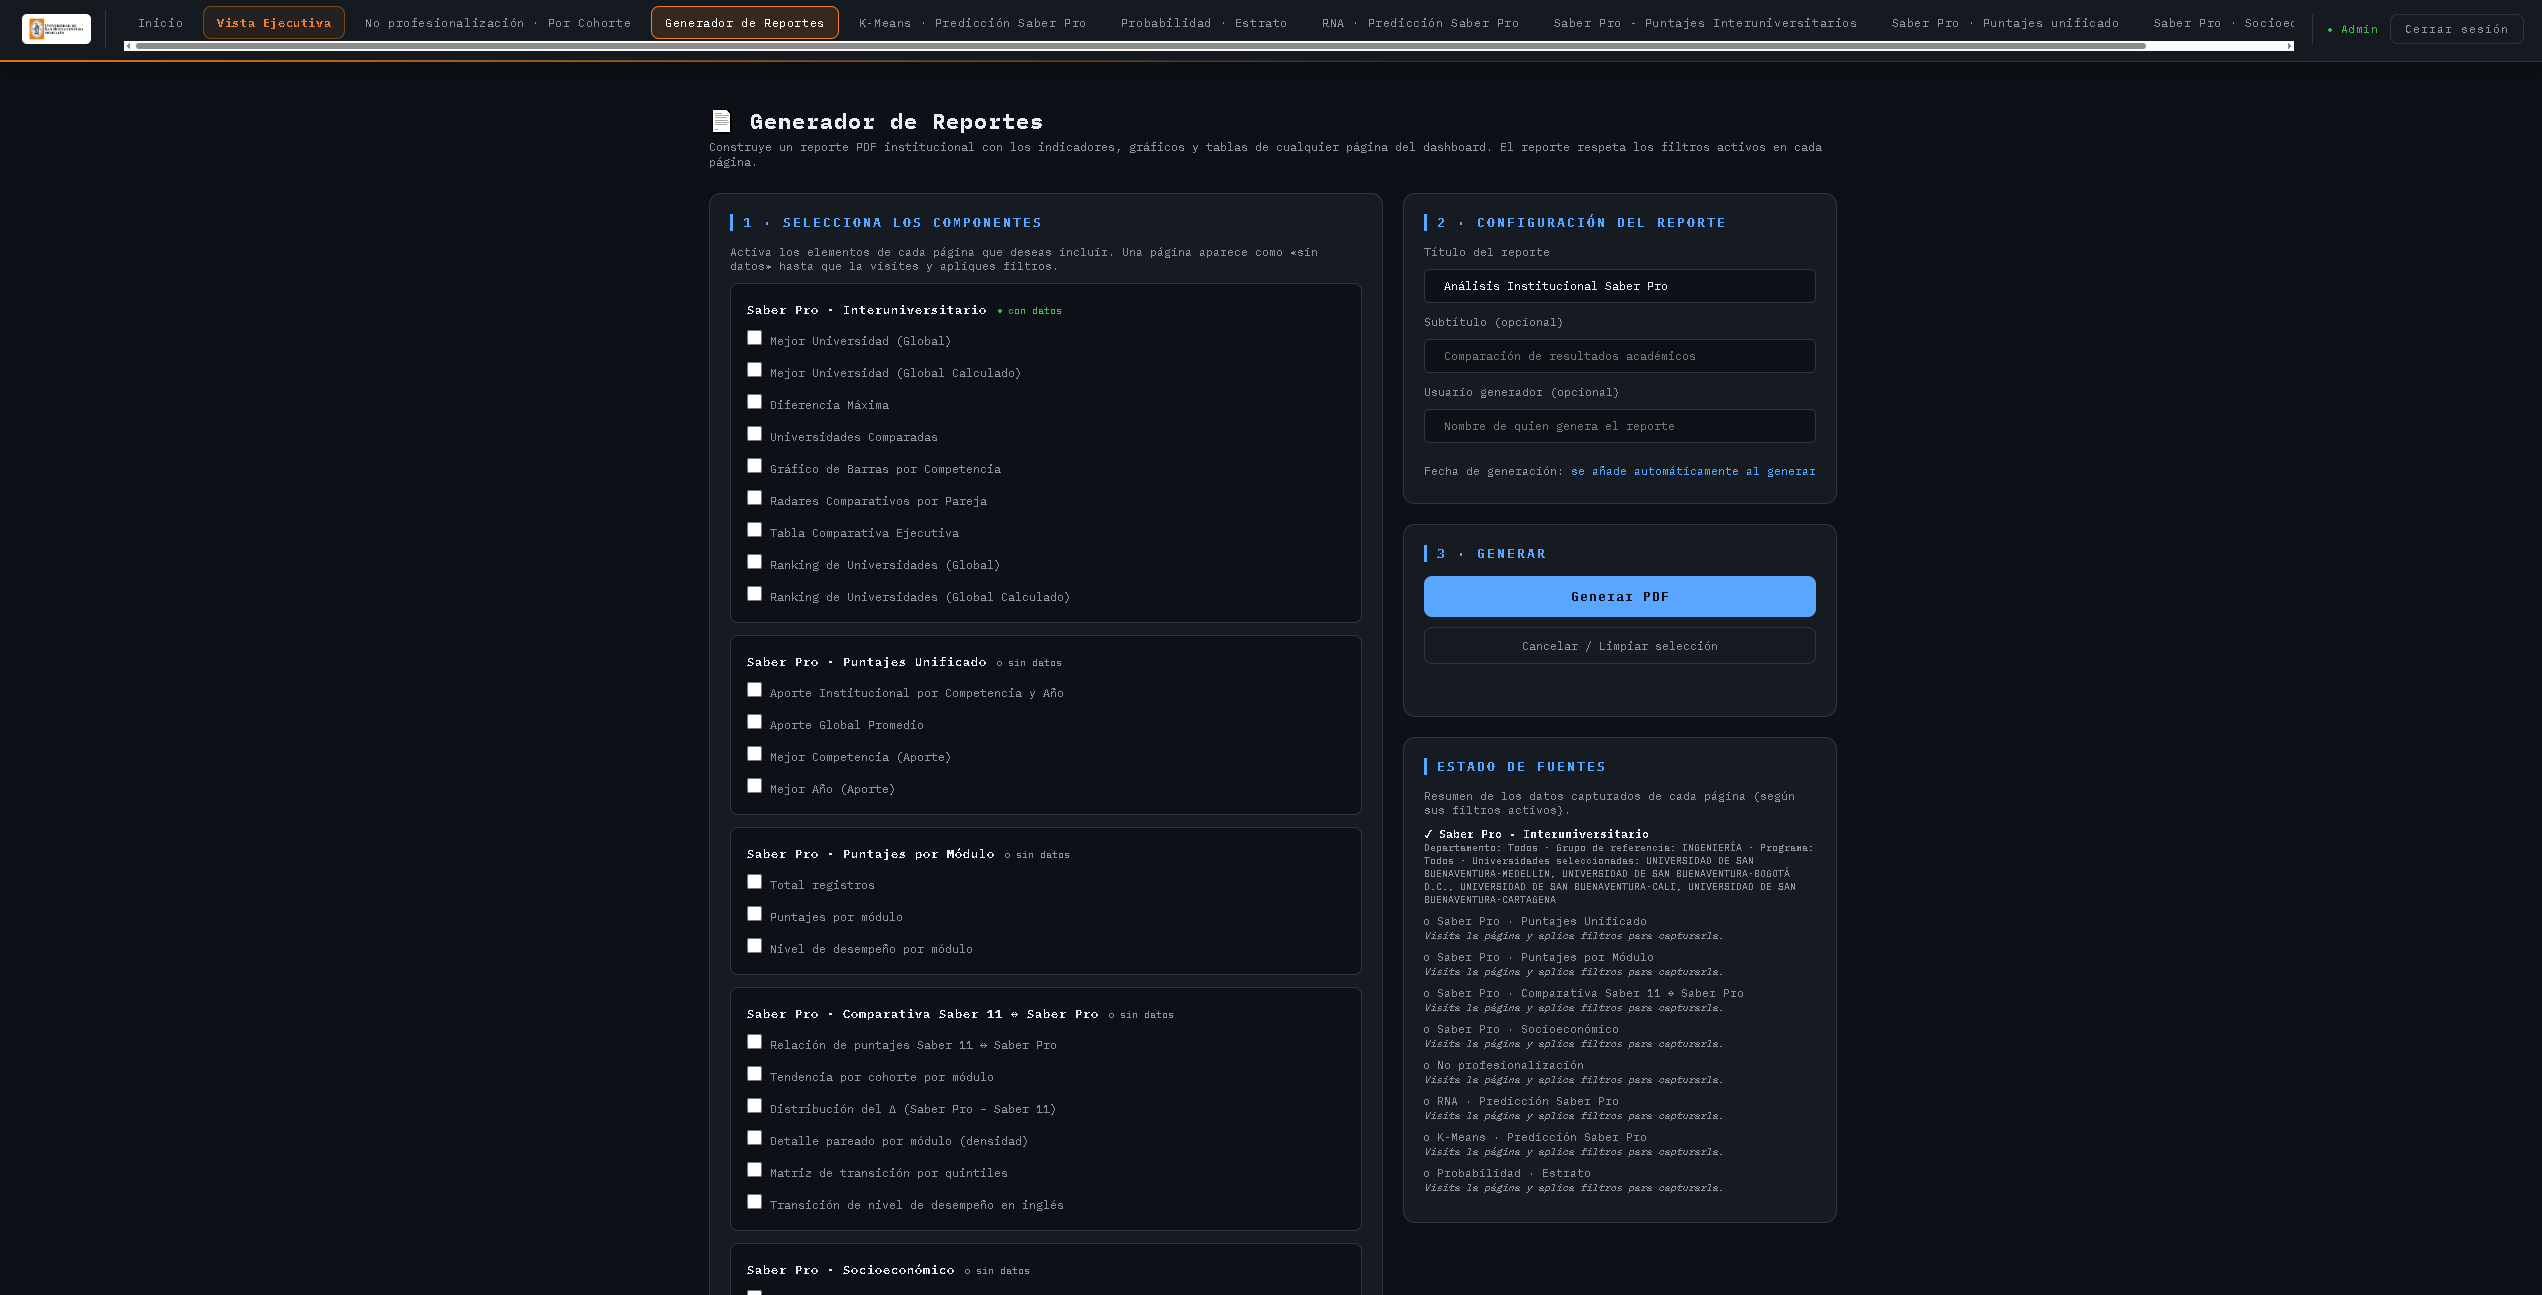
\includegraphics[width=0.7\textwidth]{images/generador_pdf.png}
	\caption{Menú para generar reportes en PDF.}
	\label{fig:mi_imagen}
\end{figure}

\begin{figure}[h]
	\centering
	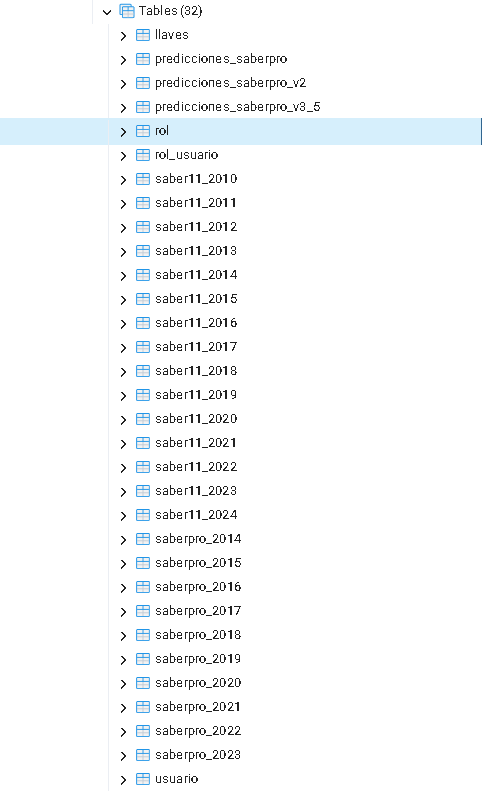
\includegraphics[width=0.7\textwidth]{images/database1.png}
	\caption{Tablas de la base de datos.}
	\label{fig:mi_imagen}
\end{figure}